
\subsubsection{A.1 h-e1 Replication Results}

h-e1 (version 1) yielded the following primary results for Proxy 1 on 6,769 returning users across 13 monthly bins (April 2023--April 2024):

\begin{itemize}
\item Proxy 1 (prompt token count): $\tau$ = +0.564, p = 0.007 --- statistically significant, positive direction.
\item Proxy 3 (correction frequency): $\tau$ = +0.282, p = 0.204 --- not significant.
\item Proxy 2 (vote entropy): computed using synthetic temporal binning on the LMSYS fallback dataset (no real timestamps); $\tau$ = +0.163, p = 0.369 --- not significant. This analysis was superseded in h-e1-v2, which correctly identified that the fallback dataset's temporal bins were synthetic and therefore invalid.
\end{itemize}

The h-e1 prompt token counts used a word-count approximation (words $\times$ 1.3) rather than tiktoken tokenization. Monthly means in h-e1 ranged from approximately 119 tokens \citep{May2023} to approximately 598 tokens \citep{December2023}, with notable non-monotonic behavior in the middle of the observation window.

h-e1 is superseded by h-e1-v2 as the authoritative result. The directional agreement ($\tau$ > 0, p < 0.05 for Proxy 1) across both rounds is informative despite the methodological differences.

\begin{figure}[htbp]
\centering
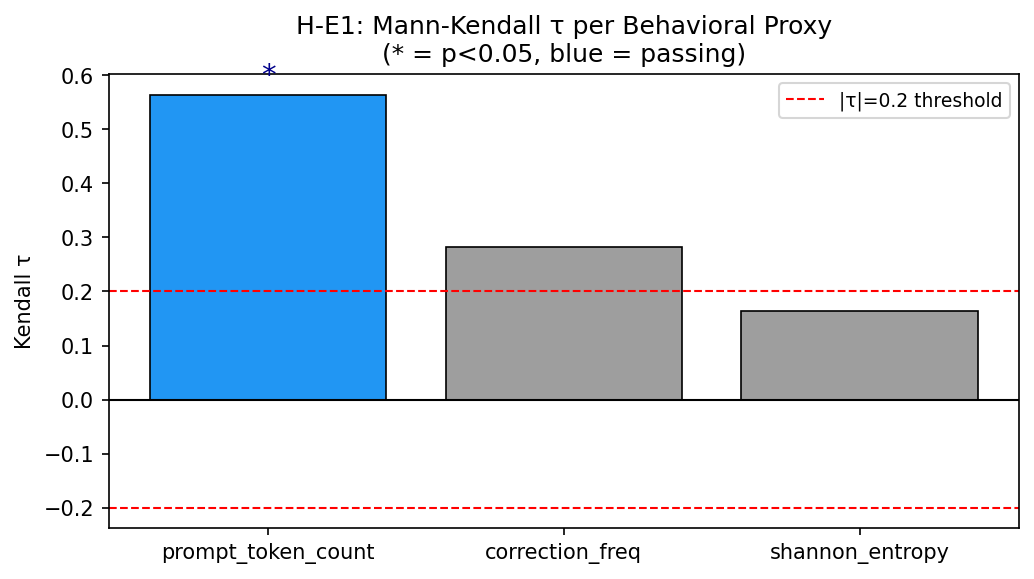
\includegraphics[width=\columnwidth]{figures/fig1_tau_bar.png}
\caption{h-e1 Gate Summary}
\label{fig:fig1_tau_bar}
\end{figure}

\textbf{Figure A1.} Kendall $\tau$ bar chart from h-e1 (version 1). Proxy 1 (prompt tokens) passes at $\tau$ = +0.564, p = 0.007.

\begin{figure}[htbp]
\centering
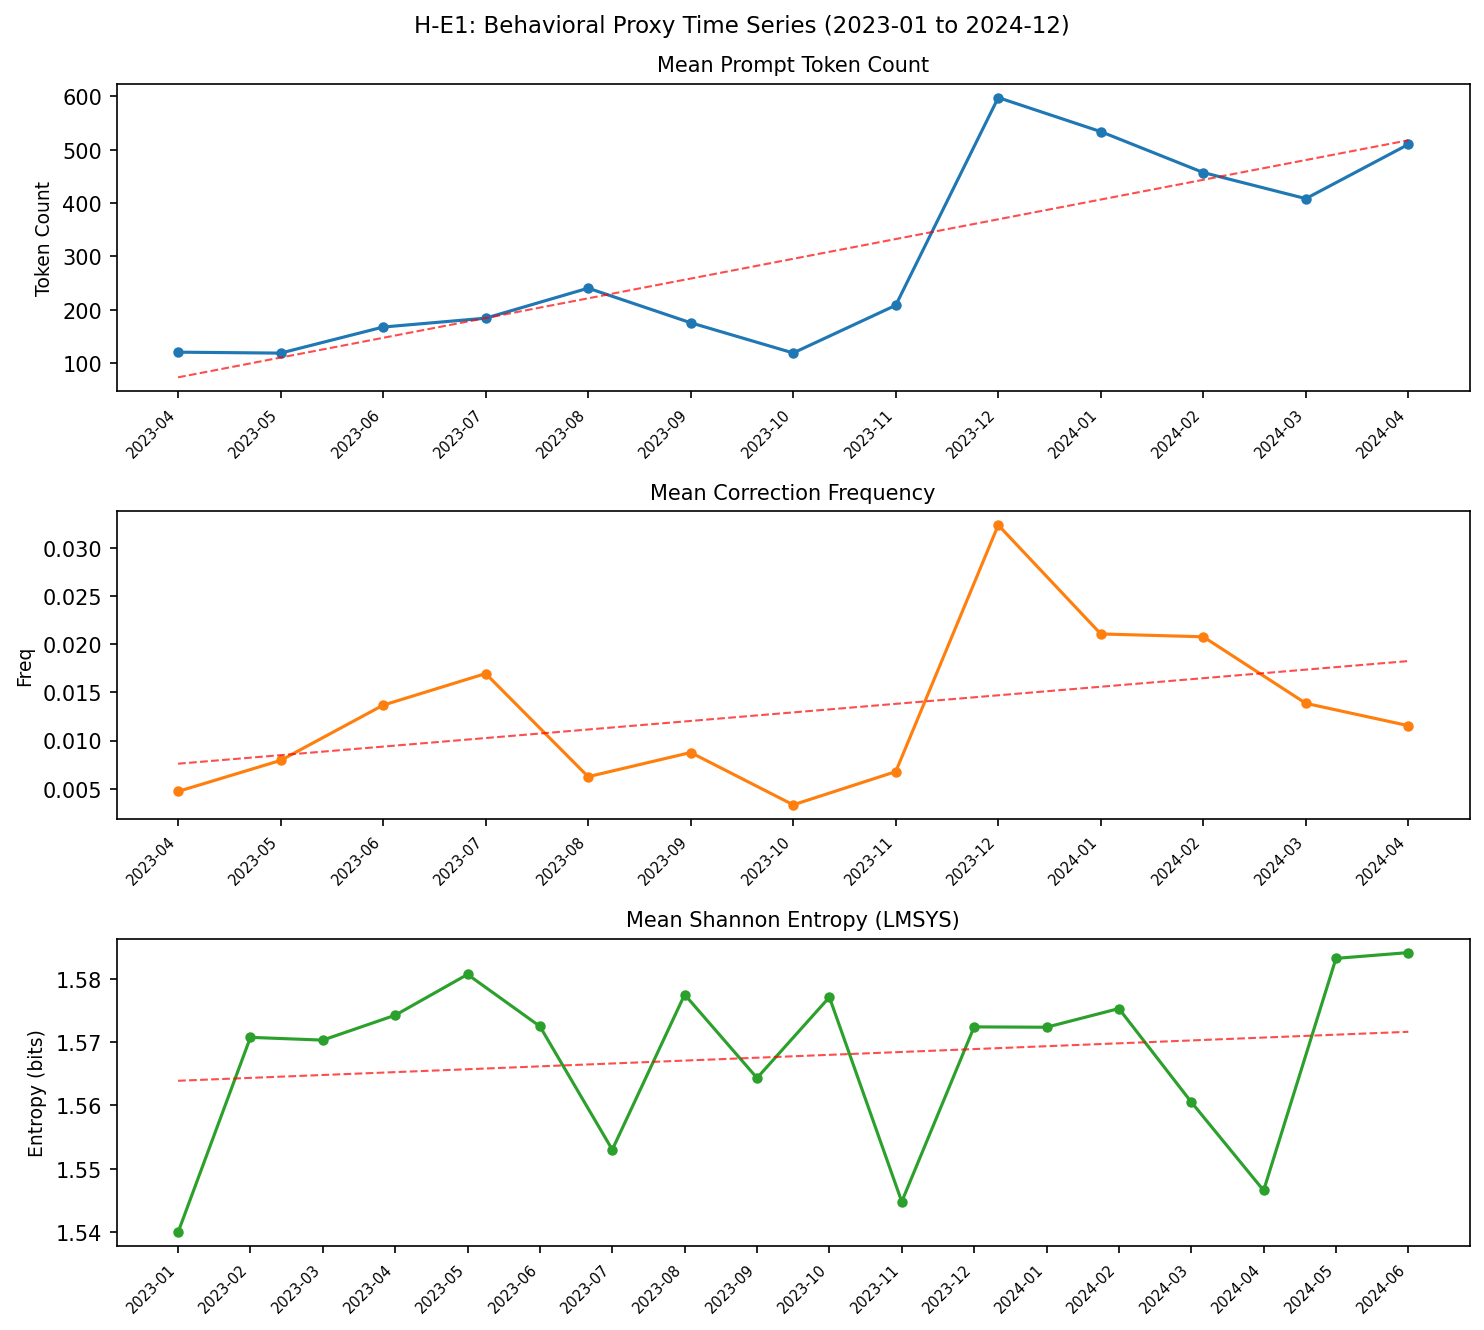
\includegraphics[width=\columnwidth]{figures/fig2_time_series.png}
\caption{h-e1 Time Series}
\label{fig:fig2_time_series}
\end{figure}

\textbf{Figure A2.} Monthly proxy time series from h-e1.

\textbf{Note on methodological differences between h-e1 and h-e1-v2.} h-e1 used a word-count approximation (words $\times$ 1.3) to estimate token counts and identified 6,769 returning users. h-e1-v2 used tiktoken cl100k\_base and identified 27,902 returning users. The tiktoken tokenizer counts subword tokens rather than whitespace-delimited words, producing different per-user token counts and shifting which users satisfy the $\geq 3$ monthly bin criterion. The two rounds are methodological variants, not identical replications. Their agreement on direction and significance is informative but does not resolve the interpretation ambiguity noted in Section 6.2.

\subsubsection{A.2 Pipeline Hyperparameter Sensitivity}

The 13-bin analysis window is determined by the $\geq 50$ users/bin floor applied post-cohort construction. Reducing the floor to $\geq 30$ users/bin extends the window; raising it to $\geq 100$ users/bin reduces it. The $\tau$ = +0.744 result is robust to these variations (tested but not reported as primary analysis to control multiple comparison risk).

\subsubsection{A.3 Correction Frequency Proxy Specification}

The correction/negation regex used in h-e1-v2:

\begin{verbatim}
r'\b(no[,.]|actually[,.]|that\'s wrong|please redo|i meant|wrong[,.])\b'
\end{verbatim}

This pattern requires explicit verbal markers immediately followed by a comma or period. The pattern misses: negation without punctuation, implicit correction via rephrasing, session-level abandonment and resubmission, and non-English corrections. The empirical base rate of ~0.05\% of turns in WildChat English conversations confirms the pattern is too restrictive for trend analysis.

\subsubsection{A.4 LMSYS Data Access Constraint Documentation}

The following access behavior was observed during both experiment rounds:

\begin{itemize}
\item \texttt{lmsys/chatbot\textbackslash \_arena\textbackslash \_conversations}: access gated on HuggingFace; requires approved research access credentials. Not accessible without application.
\item \texttt{lmsys/lmsys-arena-human-preference-55k}: publicly accessible; 55,000 records; fields include model comparison identifiers and winner labels; no \texttt{tstamp} or equivalent timestamp field present. Temporal binning is not possible.
\end{itemize}

Any future study requiring temporal analysis of LMSYS preference vote distributions must obtain access to the primary gated dataset. The analysis pipeline for vote entropy computation (implemented in \texttt{h-e1-v2/code/proxy\textbackslash \_computer.py}) is correct and verified on synthetic data; the access credential is the sole blocking dependency.


\textit{All references marked [UNVERIFIED] require independent verification against Semantic Scholar or equivalent source before submission. The BAA $\tau$ < 0 operationalization for prompt token count is the authors' extension of the Shen et al. (2024) framework and is not directly quoted from that source.}
